%!TEX root = ../operads_paper.tex
\section{Computing automorphisms of the unit}

Now we turn to the matter of computing the group $L_n(I,I)$. This group completely controls the morphisms which arise from the presence of $n$ different invertible objects as we saw in \cref{split_coh}. Our computations are necessarily of a different flavor from the theory we have so far established, since the goal has changed from establishing the existence of this group to determining it explicitly with generators and relations.

\subsection{Nullary operations}
We will begin our computational investigations by first studying the nullary operations, the elements $g \in \Lambda(0)$.

\begin{lem} \label{noscalar} Let $m \in \mathbb{N}$ and let $\ML$ be an action operad. For any element $g \in \Lambda(m)$, the morphism
  \[
    g^{\otimes} \colon  I^m \rightarrow I^m
  \]
in $L_n$ is the identity.
Equivalently, for any element $h \in \Lambda(0)$, $h$ induces the identity morphism $I \rightarrow I$.
\end{lem}
\begin{proof}
First, let $g \in \Lambda(m)$. Then $g \colon  I^m \rightarrow I^m$ is equal to $q(g) \colon q(I^m) \rightarrow q(I^m)$ which is equal to $q\delta(g) \colon  q\delta(I^m) \rightarrow q\delta(I^m)$. Since $q$ is the coequalizer of $\delta$ and the zero map, $q\delta(g) = \id$ for all $g \in \Lambda(m)$. This implies that every $h \in \Lambda(0)$ induces the identity map $I \rightarrow I$, but note that the morphism $g^\otimes \colon I^m \rightarrow I^m$ is also the morphism induced by $\mu(g; e_0, \ldots, e_0) \in \Lambda(0)$, so these two claims are equivalent.
\end{proof}

This is a curious result. The morphisms $I \rightarrow I$ in $\ELn$ are exactly the elements of the group $\Lambda(0)$, but all of these become the identity in $L_n$. In other words, $L_n$ cannot detect any morphisms in $\Lambda(0)$, an idea we make precise in the next two results. 


\begin{prop} \label{G0quot} Let $\Lambda$ be a crossed action operad. Then there exists another crossed action operad $\Lambda'$ given by $\Lambda'(m) = \Lambda(m)/\Lambda(0)$ for all $m \in \mathbb{N}$.
\end{prop}
\begin{proof}
For any elements $g \in \Lambda(m)$ and $h \in \Lambda(0)$, their block sum $h \oplus g := \mu(e_2; h, g)$ is also an element of $\Lambda(m)$. Thus block sum defines a map $\Lambda(0) \times \Lambda(m) \rightarrow \Lambda(m)$, which is a group action by operad associativity and \cref{G0abel}, and a group homomorphism by the action operad axioms and \cref{calclem}. This produces a homomorphism $- \oplus e_m \colon \Lambda(0) \rightarrow \Lambda(m)$ for all $m$, the image of which lies in the center of $\Lambda(m)$ by the action operad axioms and \cref{calclem}. Hence the image is normal for all $m$. Furthermore, the induced map $\Lambda(0) \rightarrow \Lambda(m) \rightarrow \Sigma_m$ is the zero map, so there is an induced homomorphism $\Lambda(m)/\Lambda(0) \rightarrow \Sigma_m$. All that remains to be shown is that the operadic multiplication for $\Lambda$ induces one for the groups $\Lambda(n)/\Lambda(0)$, and that this multiplication satisfies the axioms for an action operad.

Let $h, h_1, \ldots, h_m \in \Lambda(0)$ and $k_1, \ldots, k_m \in \mathbb{N}$. The following calculation uses the action operad axioms for $\Lambda$ and the fact that $\EL(\underline{1})$ is spacial so the $e_k$ commute with all elements of $\Lambda(0)$.
\begin{align*}
		\mu^{\Lambda}\left( \, h \oplus e_m \, ; \, \underline{h_i \oplus e_{k_i}}\right) &= \mu^{\Lambda}\left( \, \mu^{\Lambda}(e_2; h, e_m) \, ; \, \underline{h_i \oplus e_{k_i}} \right) \\
		&= \mu^{\Lambda}\left( \, e_2 \, ; \, \mu^{\Lambda}(h;-), \mu^{\Lambda}(e_m; \underline{h_i \oplus e_{k_i}}) \right) \\
		&= \mu^{\Lambda}(h;-)\oplus \mu^{\Lambda}\left(e_m; \underline{h_i \oplus e_{k_i}}\right) \\
		&= h \oplus h_1 \oplus e_{k_1} \oplus \cdots \oplus h_m \oplus e_{k_m} \\
		&= e_{k_1} \oplus \cdots \oplus e_{k_m} \oplus h \oplus h_1 \cdots \oplus h_m \\
		&= e_{k_1+\cdots+k_m} \oplus h \oplus h_1 \cdots \oplus h_m
\end{align*}

The above shows that the following square commutes.
\begin{center}
    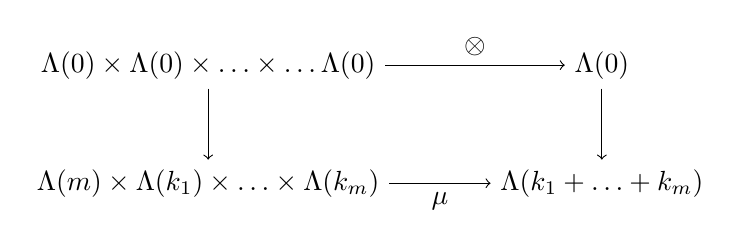
\begin{tikzpicture}[x=50mm,y=15mm]
		\node (a) at (0,0) {$ \Lambda(0) \times  \Lambda(0) \times \ldots \times \ldots  \Lambda(0)$};
		\node (b) at (1,0) {$\Lambda(0)$};
		\node (c) at (0,-1) {$ \Lambda(m) \times  \Lambda(k_1) \times \ldots \times  \Lambda(k_m) $};
		\node (d) at (1,-1) {$\Lambda(k_1 + \ldots + k_m)$};
			\draw [->] (a) to node [above] {$\otimes$} (b);
			\draw [->] (b) to node [right] {$$} (d);
			\draw [->] (a) to node [left] {$$} (c);
			\draw [->] (c) to node [below] {$\mu$} (d);
    \end{tikzpicture}
\end{center}	

We write the image of $g \in \Lambda(m)$ under the quotient $\Lambda(m) \rightarrow \Lambda'(m)$ as $[g]$. We will show that the multiplication
  \[
    \mu^{\Lambda'} \colon \Lambda'(m) \times \Lambda'(k_1) \times \cdots \times \Lambda'(k_m) \rightarrow \Lambda'(k_1 + \cdots + k_m)
  \]
given by 
  \[
    \mu^{\Lambda'}\left( [g]; [g_1], \ldots , [g_m] \right) = \left[\mu^{\Lambda}\left(g; g_1, \ldots, g_m \right)\right]
  \]
is well-defined. With $h, h_1, \ldots, h_m \in \Lambda(0)$ as above, we find that
  \[
    \mu^{\Lambda}\left(g \cdot h \otimes e_m; g_1\cdot h_1 \otimes e_{k_1}, \ldots, g_m\cdot h_m \otimes e_{k_m} \right)
  \]
equals
  \[
    \mu^{\Lambda}(g; g_1, \ldots, g_m) \cdot \mu^{\Lambda}(h \otimes e_m; h_1 \otimes e_{k_1}, \ldots, h_m \otimes e_{k_m})
  \]
using the fact that $\pi(h \otimes e_m)$ is the identity permutation. By the commutative square above, $\mu^{\Lambda}(h \otimes e_m; h_1 \otimes e_{k_1}, \ldots, h_m \otimes e_{k_m})$ is in the image of $\Lambda(0) \rightarrow \Lambda(k_1 + \cdots + k_m)$, so $\mu^{\Lambda'}$ is well-defined. It is now straightforward to check the rest of the action operad axioms for $\Lambda'$ using those of $\Lambda$.
\end{proof}

We end this section by proving that the quotient action operad $\Lambda'$ removes the unnecessary nullary operations without changing the invertible objects.

\begin{thm} \label{noscalarcross} Let $\Lambda$ be a crossed action operad, and let $\Lambda'$ be the action operad with $\Lambda'(m) = \Lambda(m)/\Lambda(0)$ constructed in \cref{G0quot}. Then for any $n \in \mathrm{N}$,
  \[
    L\ML'_n \quad \cong \quad L\ML_n
  \]
both as $\ML$-monoidal categories and as $E\Lambda'$-algebras. 
\end{thm}
\begin{proof}
The quotient map $[-] \colon \ML \rightarrow \ML'$ induces a $\ML$-algebra structure on $L\ML'_n$, and hence produces a unique strict $\ML$-monoidal functor $L\ML_n \rightarrow L\ML'_n$ by the universal property of $L\ML_n$. $L\ML_n$ is also a $\ML'$-monoidal category by defining $[g]^{\otimes} \colon x_1 \otimes \cdots \otimes x_n \rightarrow x_{[g]^{-1}1} \otimes \cdots \otimes x_{[g]^{-1}n}$ to be $g^{\otimes}$. This is well-defined, as whenever $[g] = [h]$ it is because there exists some $x \in \ML(0)$ for which $h = x \oplus g$. Then
  \[
    h^{\otimes} = (x \oplus g)^{\otimes} = x^{\otimes} \otimes g^{\otimes} = \id_I \otimes g^{\otimes} = g^{\otimes}
  \]
using \cref{otimesotimes}. Thus we also have an induced map $L\ML'_n \rightarrow L\ML_n$ using the universal property of $L\ML'_n$. By inspection, both of these functors preserve the $\ML$- and $\ML'$-actions, hence must be inverse to each other.
\end{proof}

\subsection{Reflexivity and a first calculation}

Recall that the functor $q \colon  \ELnn \rightarrow L_n$ expresses $L_n$ as a reflexive coequalizer of the morphisms $\delta, I$ of $\ML$-monoidal categories and hence also as a reflexive coequalizer of the morphisms $\tilde{\delta}, \tilde{I}$ of mere monoidal categories by \cref{q_other_coeq2}. We can therefore use the adjunction from \cref{Moradj} to calculate $\mathrm{M}(L_{n})^{\mathrm{gp, ab}}$. 

\begin{prop}\label{Zmor2} Let $\Delta$ be the subgroup of $\mathrm{M}(\ELnn)^{\mathrm{gp, ab}}$ generated by elements of the form
  \[
    \mathrm{M}(\tilde{\delta})^{\mathrm{gp, ab}}(f) \, - \, \mathrm{M}(\tilde{I})^{\mathrm{gp, ab}}(f)
  \]
for $f \in \mathrm{M}(\ELnnnn)^{\mathrm{gp, ab}}$.
Then the abelianization of the group completion of the collapsed morphisms of $L_n$ is computed as the quotient below.
  \[
    \mathrm{M}(L_{n})^{\mathrm{gp, ab}} \cong \bigquotient{{\mathrm{M}(\ELnn)}^{\mathrm{gp, ab}}}{\Delta}
  \]
\end{prop}
\begin{proof}
From \cref{Moradj}, we know that $\mathrm{M}(\, \_ \,)^{\mathrm{gp, ab}} \colon  \moncat \rightarrow \mb{Ab}$ is a left adjoint. This means that it preserves all colimits in $\moncat$, so
  \[
    \mathrm{coeq}\left( \, \mathrm{M}(\tilde{\delta})^{\mathrm{gp, ab}}, \, \mathrm{M}(\tilde{I})^{\mathrm{gp, ab}} \, \right) \cong \mathrm{M}\left( \, \mathrm{coeq}(\tilde{\delta}, \tilde{I}) \, \right)^{\mathrm{gp, ab}}.
  \]
The coequalizer of two abelian group homomorphisms is just the quotient of their common target by the image of their difference. Hence in this case we find that
  \begin{align*}
    \mathrm{M}(L_{n})^{\mathrm{gp, ab}}  &\cong \bigquotient{{\mathrm{M}(\ELnn)}^{\mathrm{gp, ab}}}{Im\left( \, {\mathrm{M}(\tilde{\delta})}^{\mathrm{gp, ab}} - {\mathrm{M}(\tilde{I})}^{\mathrm{gp, ab}} \, \right)} \\
    & \cong \quad \bigquotient{{\mathrm{M}(\ELnn)}^{\mathrm{gp, ab}}}{\Delta}.
  \end{align*}
\end{proof} 

\begin{rem}\label{delta_neq_image}
Note that $Im(\mathrm{M}(\delta)^{\mathrm{gp, ab}})$ is a subgroup of $\Delta$ because $\delta$ factors through $\tilde{\delta}$.
\end{rem}



%QQQ Rewrite with better notation

Since our goal is to be able to make explicit computations of the group acting on a set of $n$ invertible objects in a $\ML$-monoidal category, we will need an explicit description of the elements of the subgroup $\Delta$.

QQQ Started rewriting with $g^{\otimes}$ notation but this needs more time than I have now.

\begin{lem} $\Delta$ is the subgroup of $\mathrm{M}(\ELnn)^{\mathrm{gp, ab}}$ whose elements are tensor products of the equivalence classes
  \[
		\left[ \, \alpha^{\ELnn}\left( \, \mu( \, g \, ; \, e_{\left|\tilde{\delta}(x_1)\right|}, \ldots, e_{\left|\tilde{\delta}(x_m)\right|} \, ) \, ; \, \id_{x'_1}, \ldots,  \id_{x'_{m'}} \, \right) \, \right] \\
  \]
and
  \[
		\left[ \, \alpha^{\ELnn}\left( \, \mu( \, g \, ; \, e_{\left|\tilde{I}(x_1)\right|}, \ldots, e_{\left|\tilde{I}(x_m)\right|} \, ) \, ; \, \id_{x''_1}, \ldots,  \id_{x''_{m''}} \, \right) \, \right]^*
  \]
where $g \in G(m)$, the $x_i$ are generators of $\mathbb{N}^{\ast 4n}$, the $x'_i, x''_i$ are generators of $\mathbb{N}^{\ast 2n}$, and
  \begin{align*}
  	\tilde{\delta}( x_1 \otimes \ldots \otimes x_m) & =  x'_1 \otimes \ldots \otimes x'_{m'}, \\
  	\tilde{I}( x_1 \otimes \ldots \otimes x_m) & =  x''_1 \otimes \ldots \otimes x''_{m''}.
  \end{align*}
\end{lem}
\begin{proof}  
Let $f$ be an element of $\mathrm{M}(\mathbb{G}_{4n})^{\mathrm{gp, ab}}$. By definition this means that $f$ is an equivalence class of morphisms from $\mathbb{G}_{4n}$, and so by \cref{hom-set-lemma} there must exist $g \in G(m)$ and $x_1, \ldots, x_m \in \{ z_1, \ldots, z_{4n} \}$ for which
  \[
    f = \left[g^{\otimes}\right].
  \]
Thus
  \begin{align*}
		\mathrm{M}(\tilde{\delta})^{\mathrm{gp, ab}}(f) &= \mathrm{M}(\tilde{\delta})^{\mathrm{gp, ab}} \left(\,\left[g^{\otimes} \right] \,\right) \\
		&= \left[ \, \tilde{\delta}\left(g^{\otimes}\right) \, \right]  
  \end{align*}
which is $g^{\otimes}$ acting on the tensor product $\tilde{\delta}(x_1) \otimes \tilde{\delta}(x_2) \otimes \ldots \otimes \tilde{\delta}(x_n)$.
By \cref{hom-set-lemma}, we can express this isomorphism as $h^{\otimes}$ for some $h \in \Lambda(p)$ we know it must be possible to express the action morphism $\alpha^{\ELnn}(g; \id_{\tilde{\delta}(x_1)}, \ldots, \id_{\tilde{\delta}(x_m)})$ as an action morphism on the identities of generators. Since the source of this map is
  \[
    \tilde{\delta}(x_1) \otimes \ldots \otimes \tilde{\delta}(x_m) = \tilde{\delta}(x_1 \otimes \ldots \otimes x_m) =: x'_1 \otimes \ldots \otimes x'_{m'},
  \]
then the $x'_i$ are the generators we want. So by expanding the $\tilde{\delta}(x_i)$ as tensor products of these we find that
  \[
    % \left[ \, \alpha^{\ELnn}(g; \id_{\tilde{\delta}(x_1)}, \ldots, \id_{\tilde{\delta}(x_m)})  \, \right] \quad = \quad \left[ \, \alpha^{\ELnn}\left( \, \mu( \, g \, ; \, e_{|\tilde{\delta}(x_1)|}, \ldots, e_{|\tilde{\delta}(x_m)|} \, ) \, ; \, \id_{x'_1}, \ldots, \id_{x'_{m'}} \, \right) \, \right]
    \left[ \, \alpha^{\ELnn}\left(g; \underline{\id_{\tilde{\delta}(x_i)}}\right) \, \right] = \left[ \, \alpha^{\ELnn}\left( \, \mu\left( \, g \, ; \, \underline{e_{\left|\tilde{\delta}(x_i)\right|}}\, \right) \, ; \, \underline{\id_{x'_j}}\, \right) \, \right]
  \]
where
  \begin{align*}
    \underline{\id_{\tilde{\delta}(x_i)}} &= \id_{\tilde{\delta}(x_1)}, \ldots, \id_{\tilde{\delta}(x_m)}, \\
    \underline{e_{\left|\tilde{\delta}(x_i)\right|}} &= e_{|\tilde{\delta}(x_1)|}, \ldots, e_{\left|\tilde{\delta}(x_m)\right|}, \\
    \underline{\id_{x'_j}} &= \id_{x'_1}, \ldots, \id_{x'_{m'}}.
  \end{align*}
For analogous reasons we also get
\begin{align*}
			\mathrm{M}(\tilde{I})^{\mathrm{gp, ab}}(f) & = \left[ \, \alpha^{\ELnn}\left(g; \id_{\tilde{I}(x_1)}, \ldots, \id_{\tilde{I}(x_m)}\right) \, \right]  \\
			&=  \left[ \, \alpha^{\ELnn}\left( \, \mu\left( \, g \, ; \, e_{|\tilde{I}(x_1)|}, \ldots, e_{|\tilde{I}(x_m)|} \, \right) \, ; \, \id_{x''_1}, \ldots,  \id_{x''_{m''}} \, \right) \, \right]
\end{align*}
and using these equations the lemma follows immediately from the definition of $\Delta$.
\end{proof}




\subsection{Consequences of the splitting}\label{conseq_spl}

In this section we will combine our splitting result (\cref{morprod}) with the quotients in the previous section.

\begin{cor}\label{Zmor1} Let $\ML$ be a crossed action operad. Then the endomorphisms of the unit object of $L_n$ are
  \[
    L_n(I, I) \cong \bigquotient{{\MorLn}^{\ab}}{{(s \times t)(L_n)}^{\ab}}
  \]
and therefore
  \[
    \MorLn \cong (s \times t)(L_n) \, \times \, \bigquotient{{\MorLn}^{\ab}}{{(s \times t)(L_n)}^{\ab}}.
  \]
\end{cor}
\begin{proof}
Both statements follow from the simple fact that abelianization preserves products and quotients.
\end{proof}

\begin{lem} \label{colquot} Let $X$ be any monoidal category whose objects and morphisms are all invertible under tensor product (see \cref{def_tensinv} and \cref{tensinv}). Then the monoid of collapsed morphisms (see \cref{def:M}) $\mathrm{M}(X)$ is already a group, and its abelianization is isomorphic to $\mathrm{Mor}(X)^{\ab}/ \mathrm{Ob}(X)^{\ab}$.
\end{lem}
\begin{proof}
Note that both $\mathrm{Mor}(X)$ and $\mathrm{M}(X)$ are groups by assumption. Let  $f \colon  x \rightarrow y$, $f' \colon  y \rightarrow z$ be a composable pair of morphisms in $X$. Recall  that in any monoidal category with invertible objects,
  \[
    f' \circ f = f' \otimes \id_{y^{-1}} \otimes f
  \]
by \cref{tenscomp}. But $f' \otimes f = f' \circ f$ in $\mathrm{M}(X)$ by definition, so $\id_y$ is the identity element $e$ in $\mathrm{M}(X)$, and hence also $\mathrm{M}(X)^{\ab}$, for any object $y$.

Now let $A$ be an abelian group and $\phi \colon  \mathrm{Mor}(X)^{\ab} \rightarrow A$ be any homomorphism of groups which satisfies the condition $\phi(\ab(\id_x)) = e$ for all objects $x$. Then
  \begin{align*}
		\phi\left( \, \ab(f' \circ f) \, \right)  &= \phi\left( \, \ab(f' \otimes \id_{y^{-1}} \otimes f) \, \right) \\
		&= \phi\left( \, \ab(f') \, \right) \otimes \phi\left( \, \ab(\id_{y^{-1}}) \, \right) \otimes \phi\left( \, \ab(f) \, \right) \\
		&= \phi\left( \, \ab(f') \, \right) \otimes \phi\left( \, \ab(f) \, \right) \\
		&= \phi\left( \, \ab(f' \otimes f) \, \right),
	\end{align*}
but using \cref{Morder} it is easy to see that this is the defining relation for the group $\mathrm{M}(X)^{\ab}$, so $\mathrm{M}(X)^{\ab}$ and $\mathrm{Mor}(X)^{\ab}/\mathrm{Ob}(X)^{\ab}$ have the same universal property and are therefore uniquely isomorphic under $\mathrm{Mor}(X)^{\ab}$.
\end{proof}

Here is the main theorem of this section, a first description of $L_n(I,I)$.

\begin{thm}
For any crossed action operad $\ML$, 
  \[
    L_n(I,I) \cong \frac{\left(\quotient{{\mathrm{M}(\ELnn)}^{\gp,\ab}}{\Delta}\right)}{\left(\quotient{{(\mathbb{Z}^{\ast n} \times_{\mathbb{Z}^n} \mathbb{Z}^{\ast n})}^{\ab}}{\mathbb{Z}^n}\right)}, 
  \]
and the monoid of morphisms of $L_n$ is therefore
  \[ 
    \MorLn \cong \mathbb{Z}^{\ast n} \times_{\mathbb{Z}^n} \mathbb{Z}^{\ast n}  \, \times \, \frac{\left(\quotient{{\mathrm{M}(\ELnn)}^{\gp,\ab}}{\Delta}\right)}{\left(\quotient{{(\mathbb{Z}^{\ast n} \times_{\mathbb{Z}^n} \mathbb{Z}^{\ast n})}^{\ab}}{\mathbb{Z}^n}\right)}.
  \]
\end{thm}
\begin{proof}
We can make use of the isomorphism
  \[
    L_n(I,I) \cong \bigquotient{{\MorLn}^{\ab}}{{(s \times t)(L_n)}^{\ab}}
  \]
from \cref{Zmor1}. Note that this quotient  depends on the embedding of $(s \times t)(L_n)$ as a subgroup of the morphisms $L_n$ in \cref{stZsub}. The proof there ensured that the embedding we construct commutes with the inclusion of the monoid of objects, so
  \[
    \bigquotient{{\MorLn}^{\ab}}{{(s \times t)(L_n)}^{\ab}} \cong \frac{\left(\quotient{{\MorLn}^{\ab}}{\mathrm{Ob}(L_n)^{\ab}}\right)}{\left(\quotient{{(s \times t)(L_n)}^{\ab}}{\mathrm{Ob}(L_n)^{\ab}}\right)}.
  \]


Using \cref{colquot} to change the numerator and \cref{Zobj,stpullback} to simplify the denominator, this quotient becomes
  \[
    \bigquotient{{\MorLn}^{\ab}}{{(s \times t)(L_n)}^{\ab}} \cong \frac{\left(\quotient{{\mathrm{M}(\ELnn)}^{\gp,\ab}}{\Delta}\right)}{\left(\quotient{{(\mathbb{Z}^{\ast n} \times_{\mathbb{Z}^n} \mathbb{Z}^{\ast n})}^{\ab}}{\mathbb{Z}^n}\right)}
  \]
as desired.
\end{proof}

It should be clear that there is further work to do in order to give a usable construction of the category $L_n$ and the group $L_n(I,I)$. We will spend the next two sections performing the necessary algebra to interpret the complicated parts of the formula above, namely $(\mathbb{Z}^{\ast n} \times_{\mathbb{Z}^n} \mathbb{Z}^{\ast n})^{\ab}$ and ${\mathrm{M}(\ELnn)}^{\gp,\ab}$.

\subsection{Calculation: abelianizing sources and targets}
 
 Our first calculation will give a presentation for $(\mathbb{Z}^{\ast n} \times_{\mathbb{Z}^n} \mathbb{Z}^{\ast n})^{\ab}$. We were able to prove that $\mathbb{N}^{\ast n} \times_{\mathbb{Z}^N} \mathbb{N}^{\ast n}$ is a free monoid, but one cannot then conclude that $\mathbb{Z}^{\ast n} \times_{\mathbb{Z}^n} \mathbb{Z}^{\ast n}$ is a free group since group completion is a left adjoint and does not commute with pullbacks. Abelianization is also a left adjoint, and we cannot commute it past the pullback for the same reason. Thus we give a presentation directly. The algebra in this section gets rather involved. The interested reader may want to delve into the calculations here, but in any case we highlight the main results of this section now:
 \begin{itemize}
 \item we prove
  \[
    (\mathbb{Z}^{\ast n} \times_{\mathbb{Z}^n} \mathbb{Z}^{\ast n})^{\ab} \cong \mathbb{Z}^n \times {\mathbb{Z}}^{\binom{n}{2}}
  \]
 in \cref{abst} and
 \item we prove
  \[ 
    \bigquotient{{(\mathbb{Z}^{\ast n} \times_{\mathbb{Z}^n} \mathbb{Z}^{\ast n})}^{\ab}}{\mathbb{Z}^n} \cong \mathbb{Z}^{\binom{n}{2}} 
  \]
in \cref{nchoose2}.
 \end{itemize}

\begin{prop} \label{pushpres} The pullback group $\mathbb{Z}^{\ast n} \times_{\mathbb{Z}^n} \mathbb{Z}^{\ast n}$ is generated by two families of elements,
  \[
    \langle x \rangle \quad := \quad (x, x)
  \]
and
  \[
    \langle xy \rangle \quad := \quad (xy, yx)
  \]
where $x,y \in \{z_1, \ldots, z_n, z_1^*, \ldots, z_n^*\}$ are generators of the free group $\mathbb{Z}^{\ast n}$ or their inverses. These are subject to the following relations.
  \[
    \begin{array}{c}
			\langle x \rangle^{-1}  =  \langle x^* \rangle,  \quad  \langle xy \rangle^{-1}  =  \langle y^*x^* \rangle \\
			\\
			\langle xx^* \rangle  =  e  =  \langle x^*x \rangle,  \quad  \langle xx \rangle  =  \langle x \rangle^2 \\
			\\
			\langle xy \rangle \langle x^* \rangle \langle xy^* \rangle  =  \langle x \rangle \\
			\\
			\langle xy \rangle \langle x^* \rangle \langle y^* \rangle \langle yx \rangle  =  \langle x \rangle \langle y \rangle   =  \langle yx \rangle \langle x^* \rangle \langle y^* \rangle \langle xy \rangle \\
			\\
			\langle xy \rangle \langle x^* \rangle \langle xz \rangle \langle x^* \rangle \langle z^* \rangle \langle y^* \rangle \langle yz \rangle \langle y^* \rangle \langle yx \rangle \langle y^* \rangle \langle x^* \rangle \langle z^* \rangle \langle zx \rangle \langle z^* \rangle \langle zy \rangle  =  \langle x \rangle\langle y \rangle\langle z \rangle 
  	\end{array}
  \]
% Original, likely incorrect:
%       \langle xy \rangle \langle x^* \rangle \langle xz \rangle \langle x^* \rangle \langle z^* \rangle \langle y^* \rangle \langle yz \rangle \langle y^* \rangle \langle yx \rangle \langle y \rangle \langle x^* \rangle \langle z^* \rangle^{-1} \langle zx \rangle \langle z^* \rangle \langle zy \rangle  =  \langle x \rangle\langle y \rangle\langle z \rangle 
\end{prop}
\begin{proof}
\begin{itemize}
  \item QQQ Plan of the proof
  \item Describe a monoidal category: $Z$
  \item Give a `surjection' from the free $ES$-algebra on $2n$ objects, to $Z$
  \item So if we can generate the morphisms of the domain, then we can generate the morphisms of $Z$, and $Mor(Z)$ is the group we are interested in
  \item Morphisms of $S_{2n}$ are generated by identities and $\alpha((1 \, \, 2); 1,\ldots,1)$, so $Mor(Z)$ is generated by the angle-bracket generators (does the pullback being over the connected components force the pairs to be of equal length, avoiding some of the inverse issues - or even just pushing all the rewriting together at the end which would be easier, at least?)
  \item Then what relations does $Mor(Z)$ have? The ones inherited from $S_{2n}$, plus some others - how do we know we have the right ones?
\end{itemize}

We will begin by constructing a monoidal category, which we will call $Z$. The objects of $Z$ are the elements of the group $\mathbb{Z}^{\ast n}$, with the usual multiplication as the tensor product. Considering morphisms, there exists a unique morphism between any two objects $x$ and $y$ for which $\ab(x) = \ab(y)$, where $\ab \colon  \mathbb{Z}^{\ast n} \rightarrow \mathbb{Z}^n$ is the quotient map of abelianization. In other words, the morphisms of $Z$ are the elements of $\mathbb{Z}^{\ast n} \times_{\mathbb{Z}^n} \mathbb{Z}^{\ast n}$, with multiplication as the tensor product and composition given by
  \[
    (x,y) \circ (y,z)  =  (x, z).
  \]
The identity map on an object $x$ is then the unique map $(x,x) \colon x \rightarrow x$.

$Z$ is almost the subcategory of $L_n$ whose morphisms are the subgroup isomorphic to $(s \times t)(L_n)$ that we chose in \cref{stZsub}. However, we never required those representatives to be closed under composition, so $Z$ is a strictly formal version of the subcategory on $(s \times t)(L_n)$, one that doesn't involve any specific choice of the map $\rho$. It is a well-defined monoidal category; the only thing that might not be immediately clear is the law of interchange, which is just given by
  \begin{align*}
  	\left((x,y) \circ (y,z) \right) \otimes \left(  (x',y') \circ (y',z')  \right) &= (x,z) \otimes (x',z') \\
  	&= (xx',zz') \\
  	&= (xx',yy') \circ (yy',zz') \\
  	&= \left(  (x,y) \otimes (x',y')  \right) \circ \left(  (y,z) \otimes (y',z')  \right).
  \end{align*}
But now recall from \cref{tenscomp} that in any monoidal category the composition of morphisms along an invertible object can be rewritten in terms of only the tensor product. In the case of $Z$, where all of the objects have inverses, we will have
  \[
    (x,y) \circ (y, z)  =  (x, y) \otimes (y^*, y^*) \otimes (y, z).
  \]
Using this composition operation will make it easier to understand the structure of the group $\mathbb{Z}^{\ast n} \times_{\mathbb{Z}^n} \mathbb{Z}^{\ast n}$.

Next, let $\mathbb{S}_{2n}$ be the free $\mathrm{E}S$-algebra on $2n$ objects, where $S$ is the symmetric action operad. Then there exists an obvious monoidal functor $\psi \colon \mathbb{S}_{2n} \rightarrow Z$, given as follows.
  \begin{align*}
		 \psi(z_i) &= z_i \\
		 \psi(z_{n+i}) &= z_i^* \\
		 \psi(\alpha(\sigma; \id_{x_1}, \ldots, \id_{x_m})) &= (x_1 \otimes \ldots \otimes x_m, x_{\sigma(1)} \otimes \ldots \otimes x_{\sigma(m)})
	\end{align*}
A necessary condition for $(y, y')$ to be an element of $\mathbb{Z}^{\ast n} \times_{\mathbb{Z}^n} \mathbb{Z}^{\ast n}$ is that there exists some sequence of generators and their inverses $x_1, \ldots, x_m \in \{z_1, \ldots, z_n, z_1^*, \ldots, z_n^*\}$ and some permutation $\sigma \in \Sigma_m$ for which
  \begin{align*}
    y &= x_1 \otimes \ldots \otimes x_m,\\
    y' &= x_{\sigma(1)} \otimes \ldots \otimes x_{\sigma(m)}.
  \end{align*}
Hence the functor $\psi$ is surjective. It follows from this that if we can find a collection of morphisms which generate $\mathrm{Mor}(\mathbb{S}_{2n})$ under composition and tensor product, their images under $\psi$ will also generate $\mathrm{Mor}(Z) = \mathbb{Z}^{\ast n} \times_{\mathbb{Z}^n} \mathbb{Z}^{\ast n}$ under composition and tensor product, and hence under just tensor product. To begin, we know that any permutation $\sigma \in \Sigma_m$ can be written as a product $\sigma_{i_k} \cdot \ldots \cdot \sigma_{i_1}$ of elementary transpositions, giving
  \begin{align*}
  	\alpha(\sigma;\id_{x_1}, \ldots, \id_{x_m}) = &\alpha(\sigma_{i_k} \cdot \ldots \cdot \sigma_{i_1}; \id_{x_1}, \ldots, \id_{x_m}) \\
  	= &\alpha(\sigma_{i_1}; \id_{x_1}, \ldots, \id_{x_m})  \\
  	\circ &\alpha(\sigma_{i_2}; \id_{x_{\sigma_{i_1}(1)}}, \ldots, \id_{x_{\sigma_{i_1}(m)}}) \\
    \circ &\ldots \\
  	\circ &\alpha(\sigma_{i_k}; \id_{x_{\sigma_{i_{k-1}} \cdot \ldots \cdot \sigma_{i_1}(1)}}, \ldots, \id_{x_{\sigma_{i_{k-1}} \cdot \ldots \cdot \sigma_{i_1}(m)}}).
  \end{align*}
Then if $\sigma_i = \trans{i}{i+1} \in \Sigma_m$ is some elementary transposition we will have
  \begin{align*}
  	\alpha(\trans{i}{i+1} ; \id_{x_1}, \ldots, \id_{x_m} ) &= \alpha(e_{i-1} \otimes \trans{1}{2} \otimes e_{m-i-1};  \id_{x_1}, \ldots, \id_{x_m} ) \\
  	& =\id_{x_1 \otimes \ldots \otimes x_{i-1}} \otimes \alpha(\trans{1}{2};\id_{x_i}, \id_{x_{i+1}}) \otimes \id_{x_{i+2} \otimes \ldots \otimes x_m}.
  \end{align*}
Therefore all of the morphisms of $\mathbb{S}_{2n}$ are generated by just the identities and the action maps $\alpha(\trans{1}{2};\id_{x_1}, \id_{x_2})$ for all pairs $x_1, x_2 \in \{z_1, \ldots, z_{2n} \}$. Passing through $\psi$, this means that elements of $\mathbb{Z}^{\ast n} \times_{\mathbb{Z}^n} \mathbb{Z}^{\ast n}$ can always be expressed as a tensor product of elements of the form $(x, x)$ or $(x y, y x)$, where $x, y \in \{z_1, \ldots, z_n, z_1^*, \ldots, z_n^* \}$. These are exactly the $\langle x \rangle$ and $\langle xy \rangle$ given in the statement of the proposition.

Now we need to consider what relations these generators will obey. Firstly, their definitions overlap in the following case:
  \[
    \langle xx \rangle = (xx,xx) = (x,x) \otimes (x,x) = \langle x \rangle\langle x \rangle.
  \]
Next we have to account for the law of interchange we discussed earlier. Using \cref{tenscomp}, we see that this condition will induce the following relation:
  \begin{align*}
  	\langle xy \rangle \langle x^* \rangle \langle y^* \rangle \langle yx \rangle & = (xy, yx) \otimes (x^*, x^*) \otimes (y^*, y^*) \otimes (yx, xy) \\
  	& = (xy, yx) \otimes (yx, yx)^* \otimes (yx, xy) \\
  	& = (xy,yx) \circ (yx, xy) \\
  	& = (yx, xy) \otimes (yx, yx)^* \otimes (yx, xy) \\
  	& = (yx, xy) \otimes (x^*, x^*) \otimes (y^*, y^*) \otimes (xy, yx) \\
  	& = \langle yx \rangle \langle x^* \rangle \langle y^* \rangle \langle xy \rangle.
  \end{align*}
Also, by functoriality these generators will inherit any relations are obeyed to the corresponding morphisms of $\mathbb{S}_{2n}$, which in turn are just relations among different elementary transpositions. Each symmetric group $\Sigma_m$ is subject to three families of these, namely:
  \begin{align*}
  	(\sigma_i)^2 & = e, \\
  	\sigma_i \sigma_j & = \sigma_j \sigma_i, \quad j \neq i \pm 1, \\
  	(\sigma_i \sigma_{i+1})^3 & = e.
  \end{align*}
The first one, the symmetry condition, corresponds to the relation
%QQQ Unclear again. Needs writing with words, not \implies.
  \[
    \begin{array}{rrll}
      & (xy, yx) \circ (yx, xy) & = & (xy, xy) \\
      \implies & (xy, yx) \otimes (yx, yx)^* \otimes (yx, xy) & = & (x, x) \otimes (y,y) \\
      \implies & (xy, yx) \otimes (x^*, x^*) \otimes (y^*, y^*)  \otimes (yx, xy) & = & (x, x) \otimes (y,y) \\
      \implies & \langle xy \rangle\langle x^* \rangle\langle y^* \rangle\langle yx \rangle & = & \langle x \rangle\langle y \rangle. \\
    \end{array}
  \]
The second relation is just an example of interchange, which we have already considered. The third yields the fact that
  \[
    \resizebox{\textwidth}{!}{$(xy, yx)(x^*,x^*)(xz,zx)(x^*,x^*)(z^*,z^*)(y^*,y^*)(yz,zy)(y^*,y^*)(yx,xy)(y^*,y^*)(x^*,x^*)(z^*,z^*)(zx, xz)(z^*,z^*)(zy,yz)$}
  \]
is equal to $(x,x)(y,y)(z,z)$. Or simply
  \[
    \langle xy \rangle \langle x^* \rangle \langle xz \rangle \langle x^* \rangle \langle z^* \rangle \langle y^* \rangle \langle yz \rangle \langle y^* \rangle \langle yx \rangle \langle y^* \rangle \langle x^* \rangle \langle z^* \rangle \langle zx \rangle \langle z^* \rangle \langle zy \rangle = \langle x \rangle\langle y \rangle\langle z \rangle.
  \]
Finally, we need to check how the invertibility of the objects of $Z$ interacts with these generators. Most obviously,
  \begin{align*}
  	\langle x \rangle^{-1} & = (x, x)^* = (x^*, x^*) = \langle x^* \rangle, \\
  	\langle xy \rangle^{-1} & = (xy, yx)^* = (y^*x^*, x^*y^*) = \langle y^*x^* \rangle \\
  \end{align*}
and
  \begin{align*}
  	\langle xx^* \rangle & = (xx^*, x^*x)= (I, I) = e, \\
  	\langle x^*x \rangle & = (x^*x, xx^*)= (I,I) = e. \\
  \end{align*}
But we can also insert an element and its inverse into different points of the source and target:
  \begin{align*}
  	\langle x \rangle & = (x,x) \\
  	& = (xyy^*, yy^*x) \\
  	& = (xyy^*, yxy^*) \circ (yxy^*, yy^*x) \\
  	& = (xyy^*, yxy^*) \otimes (yxy^*, yxy^*)^* \otimes (yxy^*, yy^*x) \\
  	& = (xy, yx) \otimes (y^*,y^*) \otimes (y, y) \otimes (x,x)^*(y^*, y^*) \otimes (y, y) \otimes (xy^*, y^*x) \\
  	& = \langle xy \rangle \langle x^* \rangle \langle xy^* \rangle.
  \end{align*}
The relations $(xy, yx) = (zz^*xy, yzz^*x)$ and so forth are all composed of successive instance of the above, so these are all of the relations on our generators $\langle x \rangle$ and $\langle xy \rangle$.
\end{proof}

\begin{prop} \label{abst}
The groups
  $
    (\mathbb{Z}^{\ast n} \times_{\mathbb{Z}^n} \mathbb{Z}^{\ast n})^{\ab}
  $
and
  $
    \mathbb{Z}^n \times {\mathbb{Z}}^{\binom{n}{2}}
  $
are isomorphic.
\end{prop}
\begin{proof}
It follows immediately from \cref{pushpres} that the group $(\mathbb{Z}^{\ast n} \times_{\mathbb{Z}^n} \mathbb{Z}^{\ast n})^{\ab}$ has a presentation on generators
  \[
    \langle x \rangle, \langle xy \rangle, x,y \in \{z_1, \ldots, z_n, z_1^*, \ldots, z_n^*\}
  \]
subject to the following relations.
  \[
    \begin{array}{c}
    	\langle x \rangle^{-1}  =  \langle x^* \rangle,  \quad  \langle xy \rangle^{-1}  =  \langle y^*x^* \rangle \\
    	\\
    	\langle xx^* \rangle  =  e  =  \langle x^*x \rangle, \quad   \langle xx \rangle  =  \langle x \rangle^2 \\
    	\\
    	\langle xy \rangle \langle x^* \rangle \langle xy^* \rangle  =  \langle x \rangle  \\
    	\\
    	\langle xy \rangle \langle x^* \rangle \langle y^* \rangle \langle yx \rangle  =  \langle x \rangle \langle y \rangle   =  \langle yx \rangle \langle x^* \rangle \langle y^* \rangle \langle xy \rangle \\
    	\\
    	\langle xy \rangle \langle x^* \rangle \langle xz \rangle \langle x^* \rangle \langle z^* \rangle \langle y^* \rangle \langle yz \rangle \langle y^* \rangle \langle yx \rangle \langle y^* \rangle \langle x^* \rangle \langle z^* \rangle \langle zx \rangle \langle z^* \rangle \langle zy \rangle  =  \langle x \rangle\langle y \rangle\langle z \rangle 
    \end{array}
  \]
These are then also subject to the following commutativity conditions.
  \[
    \langle x \rangle \langle y \rangle = \langle y \rangle \langle x \rangle,   \langle x \rangle \langle yz \rangle = \langle z \rangle \langle xy \rangle,  	\langle wx \rangle \langle yz \rangle = \langle yz \rangle \langle wx \rangle
  \] 
Rearranging all of the former equations with the latter in mind yields the relations which follow.
  \[
    \begin{array}{c}
    	\langle x \rangle^{-1}  =  \langle x^* \rangle,  \quad  \langle xy \rangle^{-1}  =  \langle y^*x^* \rangle \\
    	\\
    	\langle xx^* \rangle  =  e  =  \langle x^*x \rangle,  \quad  \langle xx \rangle  =  \langle x \rangle^2   =  \langle xy \rangle \langle xy^* \rangle \\
    	\\
    	\langle xy \rangle \langle yx \rangle  =  \langle x \rangle^2 \langle y \rangle^2 \\
    	\\
    	\langle xy \rangle \langle yx \rangle \langle xz \rangle \langle zx \rangle \langle yz \rangle \langle zy \rangle  =  \langle x \rangle^4 \langle y \rangle^4 \langle z \rangle^4 
    \end{array}
  \]
The last of these relations is just a consequence of the one above that,
  \begin{align*}
    \langle xy \rangle \langle yx \rangle \langle xz \rangle \langle zx \rangle \langle yz \rangle \langle zy \rangle &=\left(\langle x \rangle^2 \langle y \rangle^2\right)\left(\langle x \rangle^2 \langle z \rangle^2\right)\left(\langle y \rangle^2 \langle y \rangle^2\right) \\
      &= \langle x \rangle^4 \langle y \rangle^4 \langle z \rangle^4
  \end{align*}
and in turn, the second-to-last follows from the relation above it:
  \begin{align*}
      \langle x \rangle^2 \langle y \rangle^2  &= \left(\langle xy \rangle \langle xy^* \rangle\right)\left(\langle yx \rangle \langle yx^* \rangle\right) \\
      &= \langle xy \rangle \langle yx \rangle \langle xy^* \rangle  \langle xy^* \rangle^{-1} \\
      &= \langle xy \rangle \langle yx \rangle.
  \end{align*}
Without these, we are just left with equations in two or fewer variables. Then for any two $z_i, z_j \in \mathbb{Z}^{\ast n}$, $i<j$, the first three relations tell us that we only need to consider generators of the form
  \[
    \langle z_i \rangle,  \langle z_j \rangle,  \langle z_i z_j \rangle,  \langle z_i^* z_j\rangle,  \langle z_i z_j^* \rangle,  \langle z_i^* z_j^* \rangle.
  \]
Finally, the remaining relation $\langle x \rangle^2  =  \langle xy \rangle \langle xy^* \rangle$ induces a system of four linear equations on these six generators, which can be solved to give
  \begin{align*}
			\langle z_i^* z_j \rangle &= \langle z_j \rangle^2 \langle z_i z_j \rangle^{-1}, \\
			\langle z_i z_j^* \rangle &= \langle z_i \rangle^2 \langle z_i z_j \rangle^{-1}, \\
			\langle z_i^* z_j^* \rangle &= \langle z_i \rangle^{-2} \langle z_j \rangle^{-2} \langle z_i z_j \rangle
  \end{align*}
and three independent variables: $\langle z_i \rangle$, $\langle z_j \rangle$, and $\langle z_i z_j \rangle$. In other words, $(\mathbb{Z}^{\ast n} \times_{\mathbb{Z}^n} \mathbb{Z}^{\ast n})^{\ab}$ is the free abelian group generated by elements of this form, for $1 \le i < j \le n$, which means that
  \[
    (\mathbb{Z}^{\ast n} \times_{\mathbb{Z}^n} \mathbb{Z}^{\ast n})^{\ab}  \cong  \mathbb{Z}^n \times \mathbb{Z}^{\binom{n}{2}}.
  \]
\end{proof}

From this presentation, it should be immediately obvious QQQ (Check obviousness.) how to calculate the denominator from \cref{Zmor1}.

\begin{cor}\label{nchoose2}
The following groups are isomorphic:
  \[
    \bigquotient{{(\mathbb{Z}^{\ast n} \times_{\mathbb{Z}^n} \mathbb{Z}^{\ast n})}^{\ab}}{\mathbb{Z}^n} \cong \bigquotient{\mathbb{Z}^n \times \mathbb{Z}^{\binom{n}{2}}}{\mathbb{Z}^n} \cong \mathbb{Z}^{\binom{n}{2}}.
  \]
\end{cor}
\begin{proof}
The $\mathbb{Z}^n$ term in the product of \cref{abst} represents the free abelian group generated by the morphisms
  \[
    \langle x \rangle  :=  (x,x)  =  \id_{x}.
  \]
But this is exactly the same $\mathbb{Z}^n$ group that appears in the denominator of our quotient, $\mathrm{Ob}(L_n)^{\ab}$, so they cancel.
\end{proof}

%QQQ I don't completely understand the following discussion.

Before moving on, we should be clear about exactly which $\mathbb{Z}^{\binom{n}{2}}$ subgroup of $\MLn^{\ab}$ we have just identified --- after all, we will eventually need to perform a quotient involving it. In \cref{pushpres} we defined the generators $\langle z_i z_j \rangle$ to be the elements $(z_i \otimes z_j, z_j \otimes z_i)$ of the monoid $\mathbb{Z}^{\ast n} \times_{\mathbb{Z}^n} \mathbb{Z}^{\ast n}$, which are the source/target combinations of morphisms of $L_n$. Using \cref{stZsub} we can identify this with a particular submonoid of the morphisms of $L_n$, specifically the image under $q$ of the submonoid $\mathbb{N}^{\ast 2n} \times_{\mathbb{N}^{2n}} \mathbb{N}^{\ast 2n} = (s \times t)(\ELnn) \subseteq \mathrm{Mor}(\ELnn)$ we chose in \cref{stGnsub}. In particular, since on objects $q(z_i) = z_i$ for all $1 \le i \le n$, the generators $(z_i \otimes z_j, z_j \otimes z_i)$ of $\mathbb{Z}^{\ast n} \times_{\mathbb{Z}^n} \mathbb{Z}^{\ast n}$ are clearly the image of the generators $(z_i \otimes z_j, z_j \otimes z_i)$ of $\mathbb{N}^{\ast 2n} \times_{\mathbb{N}^{2n}} \mathbb{N}^{\ast 2n}$. 

Thus, consider the following commutative diagram, whose top-left region comes from \cref{stZsub}, bottom-left from the naturality of the adjoint functor $\mathrm{M}( \, \_ \, )^{\gp,\ab}$, and right-hand square from \cref{colquot}.
% \[ \begin{tikzcd}[column sep=tiny] 
% & (s \times t)(\ELnn) \ar[dl, hookrightarrow] \ar[rr, "q"] & & (s \times t)(L\mathbb{G}_{n}) \ar[dl, hookrightarrow] \ar[dr] & \\
% \mathrm{Mor}(\ELnn) \ar[rr, "q"] \ar[dr] & & \MorLn \ar[dr] & & \frac{\displaystyle (s \times t)(L\mathbb{G}_{n})^{\ab}}{\displaystyle \mathrm{Ob}(L_n)^{\ab}} \ar[dl, hookrightarrow] \\
% & \mathrm{M}(\ELnn)^{\gp,\ab} \ar[rr, "\mathrm{M}(q)^{\gp,\ab}"] & & \MLn^{\gp,\ab}
% \end{tikzcd} \]

  \[
    \xy
      (0,0)*+{(s \times t)(\ELnn)}="a";
      (40,0)*+{(s \times t)(L\mathbb{G}_n)}="b";
      (-20,-15)*+{\mathrm{Mor}(\ELnn)}="c";
      (20,-15)*+{\MorLn}="d";
      (60,-15)*+{\frac{\displaystyle (s \times t)(L\mathbb{G}_{n})^{\ab}}{\displaystyle \mathrm{Ob}(L_n)^{\ab}}}="e";
      (0,-30)*+{\mathrm{M}(\ELnn)^{\ab}}="f";
      (40,-30)*+{\MLn^{\gp,\ab}}="g";
      %
      {\ar^{q} "a" ; "b"};
      {\ar "b" ; "e"};
      {\ar@{^{(}->} "a" ; "c"};
      {\ar@{^{(}->} "b" ; "d"};
      {\ar^{q} "c" ; "d"};
      {\ar "c" ; "f"};
      {\ar "d" ; "g"};
      {\ar_{M(q)^{\gp,\ab}} "f" ; "g"};
      {\ar@{^{(}->} "e" ; "g"};
    \endxy
  \]
What we have just said is that if we start with the element $(z_i \otimes z_j, z_j \otimes z_i)$ of $(s \times t)(\ELnn)$, moving clockwise around the diagram will send it to the generator $\langle z_i z_j \rangle$ in ${(s \times t)}(L\mathbb{G}_{n})^{\ab}/\mathrm{Ob}(L_n)^{\ab} = \mathbb{Z}^{\binom{n}{2}}$. If we instead move anticlockwise, then we will first pass to our chosen representative $\alpha_{\ELnn}(\rho(z_i \otimes z_j, z_j \otimes z_i); \id_{z_i}, \id_{z_j})$ in $\mathrm{Mor}(\ELnn)$, then its equivalence class in $\mathrm{M}(\ELnn)^{\gp,\ab}$, then its equivalence class in $\MLn^{\gp,\ab}$, using the fact that $\mathrm{M}(q)^{\gp,\ab}$ is the canonical map associated with the quotient
  \[
    \MLn^{\mathrm{gp, ab}} = \bigquotient{{\mathrm{M}(\ELnn)}^{\mathrm{gp, ab}}}{\Delta}
  \]
which we proved in \cref{Zmor2}. Since the bottom-right inclusion completes this circuit, we see that the specific subgroup in \cref{nchoose2} is
  \[
    \mathbb{Z}^{\binom{n}{2}} = \big\{\left[\alpha_{\ELnn}\left(\rho(z_i \otimes z_j, z_j \otimes z_i); \id_{z_i}, \id_{z_j} \right) \right] : 1 \le i < j \le n \big\} \subseteq \MLn^{\ab}.
  \]

Of course, $\rho$ was an arbitrary permutation-preserving map $\mathbb{N}^{\ast n} \times_{\mathbb{N}} \mathbb{N}^{\ast n} \rightarrow G$, chosen using the freeness of its source monoid. Thus if we wanted to we could just pick the same element $\rho(2) \in \pi^{-1}(\trans{1}{2})$ to act as $\rho(z_i \otimes z_j, z_j \otimes z_i)$ for all $i, j$. For simplicity's sake, we will indeed be assuming this from now on.

\subsection{Calculation: collapsed morphisms}

The next group we are interested in understanding better is $\mathrm{M}(\ELnn)^{\gp,\ab}$. By \cref{Morder}, the operations needed to produce this group from
  \[
    \mathrm{Mor}(\ELnn) = \ML \times_{\mathbb{N}} \mathbb{N}^{\ast 2n}
  \]
can be done in any order we choose, and so we will save the identification of $\otimes$ and $\circ$ until last. This will let us keep the tensor product as simple as possible while we are in the process of group completing and abelianizing it. We begin with group completion, using a method developed by Raouf Doss \cite{doss-imm}.

\begin{Defi} We say that a monoid $M$ is \emph{left-cancellative} if for any $a, b, c \in M$, then
  \[
    ab = ac \implies b = c.
  \]
That is, common factors may be cancelled out on the left. Similarly, we call $M$ \emph{right-cancellative} if common factors can be cancelled on the right:
  \[
    ac = bc \implies a = b.
  \]
A monoid that is both left- and right-cancellative is simply referred to as \emph{cancellative}.
\end{Defi}

\begin{Defi} An element $a$ of a monoid $M$ is said to be \emph{regular on the left} if it shares a common left-multiple with every other element of $M$. That is, for all $b \in M$, there exists $c, d \in M$ such that $ca = db$. The monoid itself is said to be \emph{regular on the left} if all of its elements are. A similar condition can be given to describe elements and monoids which are \emph{regular on the right}.

A monoid $M$ is \emph{quasi-regular on the left} if any two elements $a,b$ of $M$ share a common left-multiple ($ca = db$ as above) if and only if there exists $c', d' \in M$ such that $c'a = d'b$ where $c'$ or $d'$ is regular in $M$. A similar condition can be given to describe a monoid which is \emph{quasi-regular on the right}. A monoid is \emph{quasi-regular} when it is both.
\end{Defi}

\begin{prop}[\cite{doss-imm}] If a monoid $M$ is cancellative and quasi-regular on the left, then it can be embedded into a group.
\end{prop}

For a given action operad, both of these conditions will follow from the way that operadic multiplication interacts with the elements of the abelian group $\Lambda(0)$.

%QQQ New notation: $\Lambda^{\oplus}$ is the monoid associated to an action operad

\begin{prop} \label{cqr} For every action operad $\ML$, the monoid $\Lambda^{\oplus}$ is both cancellative and quasi-regular as a monoid under tensor product.
\end{prop}
\begin{proof}
Let $g$ and $g'$ be any elements of $\Lambda$ which share a left-multiple, so that there exists at least one pair $h, h'$ in $\Lambda$ for which
  \[
    h \otimes g = h' \otimes g',
  \]
and without loss of generality assume that $|g| \ge |g'|$, so necessarily $|h| \le |h'|$ (see \cref{def:length}). The operadic product $\mu(h; e_0, \ldots, e_0)$ is an element of the group $\LL(0)$, and we know from \cref{G0abel} that $\LL(0)$ is an abelian group under tensor product, so let $\mu(h; e_0, \ldots, e_0)^*$ be its inverse. Then
  \begin{align*}
		g &= \mu(h; e_0, \ldots, e_0)^* \otimes \mu(h; e_0, \ldots, e_0) \otimes \mu(g; e_1, \ldots, e_1) \\
		&= \mu(h; e_0, \ldots, e_0)^* \otimes \mu\left( e_2 ; \mu(h; e_0, \ldots, e_0), \mu(g; e_1, \ldots, e_1) \right) \\
		&= \mu(h; e_0, \ldots, e_0)^* \otimes \mu\left( \mu(e_2; h, g) ; e_0, \ldots, e_0, e_1, \ldots, e_1 \right) \\
		&= \mu(h; e_0, \ldots, e_0)^* \otimes \mu\left( h \otimes g ; e_0, \ldots, e_0, e_1, \ldots, e_1 \right) \\
		&= \mu(h; e_0, \ldots, e_0)^* \otimes \mu\left( h' \otimes g' ; e_0, \ldots, e_0, e_1, \ldots, e_1 \right) \\
		&= \mu(h; e_0, \ldots, e_0)^* \otimes \mu\left( \mu(e_2; h', g') ; e_0, \ldots, e_0, e_1, \ldots, e_1 \right) \\
		&= \mu(h; e_0, \ldots, e_0)^* \otimes \mu\left( e_2 ; \mu(h'; e_0, \ldots, e_0, e_1, \ldots, e_1), \mu(g'; e_1, \ldots, e_1) \right) \\
		&= \mu(h; e_0, \ldots, e_0)^* \otimes \mu(h'; e_0, \ldots, e_0, e_1, \ldots, e_1) \otimes \mu(g'; e_1, \ldots, e_1) \\
		&= \left( \mu(h; e_0, \ldots, e_0)^* \otimes \mu(h'; e_0, \ldots, e_0, e_1, \ldots, e_1) \right) \otimes g' \\
		&=: k \otimes g'.
	\end{align*}
Put another way, if $h \otimes g = h' \otimes g'$, there exists $k \in \ML$ such that $g = k \otimes g'$, or equivalently $e_0 \otimes g = k \otimes g'$. Since $e_0$ is obviously regular because it is the unit, the operad $\LL$ viewed as a monoid is quasi-regular on the left; quasi-regularity on the right is analogous. Furthermore, following through the argument above when $h = h'$ shows that $h \otimes g = h \otimes g'$ implies $g = g'$, or left-cancellativity.
\end{proof}

\begin{cor} \label{gpcompin} The canonical map $\gp \colon \Lambda^{\oplus} \rightarrow \Lambda^{\oplus, \gp}$ associated with the group completion of $\ML$ is an inclusion. Further, the canonical map
  \[
    \gp \colon \Lambda^{\oplus} \times_{\mathbb{N}} \mathbb{N}^{\ast n} \rightarrow (\Lambda^{\oplus} \times_{\mathbb{N}} \mathbb{N}^{\ast n})^{\gp}
  \]
is also an inclusion.
\end{cor}
\begin{proof}
The first statement is immediate. For the second, note that both $\ML$ and $\mathbb{N}^{\ast n}$ embed into groups so their product and hence any submonoid of their product does too.
\end{proof}

As a consequence, we can identify the monoids $\ML$ and $\ML\times_{\mathbb{N}} \mathbb{N}^{\ast n}$ with their images in the group completion. Further, recall from \cref{noscalarcross} that for studying invertible objects, it suffices to study action operads $\ML$ with $\Lambda(0)$ the trivial group.

\begin{prop}\label{Gfree}
Let $M$ be a monoid with unit element $1$, and assume $M$ is equipped with a monoid homomorphism $\pi \colon  M \rightarrow (\mathbb{N}, +)$ such that 
\begin{itemize}
\item $\pi^{-1}(0) = \{1\}$, and
\item if $hg = h' g'$ in $M$, then there exists a $k \in M$ such that $g = kg'$, $h' = hk$.
\end{itemize}
Then $M$ is a free monoid.
\end{prop}
\begin{proof}
Let $\mathcal{G}$ be a subset of the monoid $M$, and $\mathcal{R}$ a collection of relations on the elements of $\mathcal{G}$, such that $(\mathcal{G},\mathcal{R})$ is a presentation of $M$ as a monoid. We assume that $1 \notin \mathcal{G}$ as it is the unit element. Notice that every relation in $\mathcal{R}$ can be written in the form $h g = h' g'$, where $g,g' \in \mathcal{G}$ are generators because the only other kind of relations are those for which one side of the relation is just the identity element 1, and  this is not possible if $\pi^{-1}(0) = \{1\}$. 
 
We say that a non-identity element $x \in M$ is \emph{irreducible} if whenever $x = yz$ then $y=1$ or $z=1$. (Note that $M$ contains no non-identity, left or right invertible elements: if $x, y \in M$ satisfy $xy = 1$, then $\pi(x) + \pi(y) = 0$ which then shows that $\pi(x) = \pi(y) = 0$, and thus by the first hypothesis $x = y = 1$.) Let $\mathcal{I} \subseteq M$ denote the set of all irreducible elements. We first check that $\mathcal{I}$ generates $M$. Given $x \in M$, if it is not irreducible then it admits a factorization $x = yz$ into two non-identities. Since $\pi^{-1}(0) = \{1\}$, we find that $\pi(y), \pi(z) < \pi(x)$ and QQQ (check induction argument) induction finishes the argument that every element is a product of irreducibles. Let $\mathcal{R}$ be a set of relations such that $(\mathcal{I}, \mathcal{R})$ is a presentation for $M$. Let $x_1 x_2 \cdots x_n = y_1 y_2 \cdots y_m$ be a relation in $\mathcal{R}$. Then there exists  $k \in M$ such that $x_n = k y_m$ and $x_1 x_2 \cdots x_{n-1} k = y_1 y_2 \cdots y_{m-1}$. By irreducibility of $x_n, y_m$ we must have $k=1$, so $x_n = y_m$ and $x_1 x_2 \cdots x_{n-1} = y_1 y_2 \cdots y_{m-1}$. Induction then shows that $n=m$ and $x_i = y_i$ for all $i$, so this relation is actually of the form $x_1 x_2 \cdots x_n =x_1 x_2 \cdots x_n$ and can therefore be removed from $\mathcal{R}$ without changing $M$. Since the relation was arbitrary, the presentation $(\mathcal{I}, \emptyset)$ also gives $M$, so $M$ is free.
\end{proof}
\begin{cor}\label{cor:ML_free}
If $\ML$ is an action operad with trivial $\Lambda(0)$, then $\Lambda^{\oplus}$ is a free monoid under block sum.
\end{cor}
\begin{proof}
This follows immediately from \cref{Gfree} and the arguments in the proof of \cref{cqr}.
\end{proof}

%QQQ Need to make sure we are using the correct notation: the operad, the monad, the monoid, etc

We can now use these results to describe the monoid $\mathrm{Mor}(\ELn)$ using generators for the action operad $\ML$.

\begin{prop} \label{freemor} Assume that $\ML$ is an action operad with $\LL(0)$ the trivial group. Let $\mathcal{G}$ be a set that freely generates the action operad $\ML$ under block sum, and for each $m \in \mathbb{N}$ define $\mathcal{G}_m := \mathcal{G} \, \cap \,  \Lambda(m)$, the subset of $\mathcal{G}$ containing all elements of length $m$. Then the monoid $\mathrm{Mor}(\ELn)$ is 
  \[
    \ML \times_{\mathbb{N}} \mathbb{N}^{\ast n} \cong \mathbb{N}^{\ast (n|\mathcal{G}_1| + n^2 |\mathcal{G}_2| + \ldots)}.
  \]
\end{prop}
\begin{proof}
Let $(g, w)$ be an arbitrary element of $\ML \times_{\mathbb{N}} \mathbb{N}^{\ast n}$. The monoid $\ML$ is free of the generators $\mathcal{G}$, and $\mathbb{N}^{\ast n}$ is free on $\{z_1, \ldots, z_n\}$, so we can find unique expansions of $g$ and $w$ as the following block sums and products, respectively.
  \[
    \begin{array}{ll}
			g = g_1 \oplus \ldots \oplus g_k & g_1, \ldots, g_k \in \mathcal{G} \\
			w = x_1  \ldots x_m & x_1, \ldots, x_m \in \{z_1, \ldots, z_n\}
  	\end{array}
  \]
But each of the generators $z_1, \ldots, z_n$ has length 1, so the index $m$ here is really just the length $|w|$, which by the definition of $\ML \times_{\mathbb{N}} \mathbb{N}^{\ast n}$ is also the length $|g| = |g_1| + \ldots + |g_k|$. For an element $x_1  \ldots x_m$ and $i < j$, write $x_i^j$ for the product $x_i x_{i+1} \cdots x_j$. Therefore we may write
  \begin{align*}
  	(g, w) & = \left(g_1 \oplus \ldots \oplus g_k, x_1  \ldots  x_{|w|}\right) \\
  	& = \left(g_1, x_1^{|g_1|}\right)  \left(g_2, x_{|g_1|+1}^{|g_1|+|g_2|}\right)  \ldots  \left(g_k, x_{\left(\sum_{i=1}^{k-1}|g_i| \right)+1}^{\sum_{i=1}^{k}|g_i| }\right).
  \end{align*}
That is, every element in $\ML \times_{\mathbb{N}} \mathbb{N}^{\ast n}$ may be expressed as a product of elements from the subset $\mathcal{G} \times_{\mathbb{N}} \mathbb{N}^{\ast n}$. Furthermore, the freeness of both $\ML$ and $\mathbb{N}^{\ast n}$ ensure that this expansion is unique, so $\ML \times_{\mathbb{N}} \mathbb{N}^{\ast n}$ is the free monoid on the set 
  \begin{align*}
    \mathcal{G} \times_{\mathbb{N}} \mathbb{N}^{\ast n} &= \mathcal{G}_0 \times \{ z_1, \ldots, z_n \}^0  \cup \mathcal{G}_1 \times \{ z_1, \ldots, z_n \}^1 \cup \mathcal{G}_2 \times \{ z_1, \ldots, z_n \}^2 \cup \ldots \\
    &= \bigcup_{i \in \mathbb{N}} \mathcal{G}_i \times \{z_0, \ldots, z_n\}^i.
  \end{align*}
We note that $\mathcal{G}_0$ is necessarily empty since $\LL(0)$ is trivial, and the result follows.
\end{proof}

This makes computing the group completion and abelianization trivial. 

\begin{cor} \label{freemorgpab} Assume that $\ML$ is an action operad with $\LL(0)$ the trivial group. If $\mathcal{G}$ is a set that freely generates $\ML$ under block sum, and $\mathcal{G}_m := \mathcal{G} \, \cap \,  \Lambda(m)$, then the abelian group $\mathrm{Mor}(\ELn)^{\gp, \ab}$ is 
  \[
    (\ML \times_{\mathbb{N}} \mathbb{N}^{\ast n})^{\gp, \ab} = \mathbb{Z}^{ n|\mathcal{G}_1| + n^2 |\mathcal{G}_2| + \ldots}.
  \]
\end{cor}

If we use a subset $\mathcal{G}' \subseteq \mathcal{G}$ which generates $\ML$ using both the block sum and group multiplication, then we can reduce the number of generators even further.

\begin{cor} Assume that $\ML$ is an action operad with $\LL(0)$ the trivial group. Let $\mathcal{G}$ be a subset of the action operad $\ML$ that freely generates it under block sum, and let $\mathcal{G'}$ be a subset of $\mathcal{G}$ which generates $\ML$ under a combination of block sum and group multiplication. Also let $\mathcal{G}_m := \mathcal{G} \, \cap \,  G(m)$ and $\mathcal{G}'_m := \mathcal{G}' \, \cap \,  G(m)$. Then the groups
% QQQ Changed this to say that the groups are isomorphic so it's actually a sentence. (Are they groups or monoids?)
  \[
    \bigquotient{\mathbb{Z}^{n|\mathcal{G}_1| + n^2 |\mathcal{G}_2| + \ldots}}{\otimes \sim \circ}
  \]
  and
  \[
    \bigquotient{\mathbb{Z}^{n|\mathcal{G}'_1| + n^2 |\mathcal{G}'_2| + \ldots}}{\otimes \sim \circ}
  \]
are isomorphic.
\end{cor}
\begin{proof}
Composition in $\ELn$ is given by group multiplication (when defined) by the formula
  \[
    \left( \, g', \pi\left(g^{-1}\right)(w) \, \right) \, \circ \, (g, w) = \left(g'g, w\right).
  \]
Therefore any generator $(g, w) \in \mathcal{G} \times_{\mathbb{N}} \mathbb{N}^{\ast n}$ can be expressed in terms of elements of $\mathcal{G}' \times_{\mathbb{N}} \mathbb{N}^{\ast n}$ by way of block sum and group multiplication. After making the identification $\otimes \sim \circ$ we obtain the desired isomorphism.
\end{proof}

\subsection{A full description of \texorpdfstring{$L_n$}{L_n}}\label{full_des}

We now give our most complete description of the free $\ML$-monoidal category generated by $n$ invertible objects. We know that an arbitrary morphism of $L_n$ can be described using its source, target, and an element of $L_n(I,I)$. We use this knowledge, together with a chosen isomorphism $\MorLn \cong (s \times t)(L_n) \times L_n(I,I)$, to write down $L_n$ as a $\ML$-monoidal category.

\begin{conv}
Recall that we have fixed an isomorphism 
  \[
    \MorLn \cong (s \times t)(L_n) \times L_n(I,I)
  \]
 as per \cref{morprod}. Further, assume that $\Lambda(0)$ is the trivial group; if not, replace $\Lambda$ with the action operad $\Lambda'$ of \cref{noscalarcross}.
\end{conv}

\begin{Defi} \label{AGndef} Let $\ML$ be a crossed action operad. Choose a subset $\mathcal{G}'$ that generates $\ML$ under a combination of tensor product and group multiplication, which itself has subsets $\mathcal{G}'_m := \mathcal{G}' \, \cap \, \Lambda(m)$. Then for each $n \in \mathbb{N}$, we will denote by $A(\ML,n)$ the abelian group obtained from the free abelian group 
  \[
    \mathrm{F}\left( \mathcal{G}' \times_{\mathbb{N}} \mathbb{N}^{\ast 2n}\right) = \mathbb{Z}^{2n|\mathcal{G}'_1| + (2n)^2|\mathcal{G}'_2| + \ldots}
  \]
via the following steps:
\begin{enumerate}
\item For all $g, g' \in \mathcal{G}'_m$ and $w \in \mathbb{N}^{\ast 2n}$ with $|w| = m$, quotient out by the relation 
  \[
    (g, w) \, \otimes \, \left( \, g', \pi(g^{-1})(w) \, \right) \sim (g \cdot g', w).
  \]
\item Quotient out by the subgroup $\Delta$, which is generated by the equivalence classes of elements of the form
  \[
    \begin{array}{c}
  		\left( \, \mu( \, g \, ; \, e_{|\tilde{\delta}(x_1)|}, \ldots, e_{|\tilde{\delta}(x_m)|} \, ), \, \tilde{\delta}( \, x_1 \otimes \ldots \otimes x_m \, ) \, \right) \\
  		\otimes \\
  		\left( \, \mu( \, g \, ; \, e_{|\tilde{I}(x_1)|}, \ldots, e_{|\tilde{I}(x_m)|} \, ), \, \tilde{I}( \, x_1 \otimes \ldots \otimes x_m \, ) \, \right)^*
  	\end{array} 
  \]
QQQ Change x's to z's? Just the next one, then it makes sense.
where $g \in \LL(m)$, the $x_i$ are generators of $\mathbb{N}^{\ast 4n}$, and for all $1 \le i \le n$,
  \[
    \begin{array}{ll}
  		\tilde{\delta}(z_i) = z_i, & \tilde{\delta}(z_{2n+i}) = z_i \otimes z_{n+i}, \\
  		\tilde{\delta}(z_{n+i}) = z_{n+i}, & \tilde{\delta}(z_{3n+i}) = z_{n+i} \otimes z_i, \\
      \tilde{I}(z_i) = z_i, & \tilde{I}(z_{2n+i}) = I,\\
      \tilde{I}(z_{n+i}) = z_{n+i}, & \tilde{I}(z_{3n+i}) = I.
  	\end{array}
  \] 
\item Choose any $\rho(2) \in \pi^{-1}(\trans{1}{2})$, and then quotient out by the $\mathbb{Z}^{\binom{n}{2}}$ subgroup generated by the equivalence classes of the elements 
  \[
    \left(\rho(2) ;z_i, z_j \right), 1 \le i < j \le n.
  \]
\end{enumerate}
We write $\Psi \colon  \ML^{\oplus} \times_{\mathbb{N}} \mathbb{N}^{\ast 2n} \rightarrow A(\ML,n)$ to represent the corresponding quotient map. 
\end{Defi}

\begin{example}
As an example, for the symmetric operad $\Sigma$, we can take $\mathcal{G}'_m$ to be empty for $m \neq 2$ and the singleton set $\{ \trans{1}{2} \}$ for $m=2$. We return to this example, and others, in the next chapter.
\end{example}

With this new notation, we complete the computation of the free $\ML$-monoidal category on $n$ invertible objects in the theorem below.

\begin{thm}\label{freeinvalgc} Let $\ML$ be a crossed action operad. Then the free $\ML$-monoidal category on $n$ invertible objects is the category
  \[
    L_n \cong \mathbb{Z}^{\ast n} \times_{\mathbb{Z}^n} \mathbb{Z}^{\ast n}  \, \times \, \mathrm{B}A(\ML,n)
  \]
equipped with the componentwise monoidal structure,
  \[
    (x', y' ,h') \otimes (x, y, h) = (x' \otimes x, y' \otimes y, h'h)
  \]
and the $E\Lambda$-action given in \cref{crossact}:
  \[
    \begin{array}{c}
			\alpha_{L_n}\left(g;(x_1, y_1, h_1), \ldots, (x_m, y_m, h_m) \right) \\
			= \\
			\left(\bigotimes_i x_i, \bigotimes_i y_{\pi(g^{-1})(i)}, \Psi \alpha_{\ELnn}\left(g;\id_{q^{-1}(y_1)}, \ldots, \id_{q^{-1}(y_m)}\right) \otimes \left(\bigotimes_i h_i\right)\right) 
  	\end{array}
  \]
\end{thm}
\begin{proof}
The category $\mathbb{Z}^{\ast n} \times_{\mathbb{Z}^n} \mathbb{Z}^{\ast n} \times \mathrm{B}A(\ML,n)$ is just the one which has objects $\mathbb{Z}^{\ast n} \times_{\mathbb{Z}^n} \mathbb{Z}^{\ast n}$, morphisms $\mathbb{Z}^{\ast n} \times_{\mathbb{Z}^n} \mathbb{Z}^{\ast n} \times A(\ML,n)$, and composition 
  \[
    (y, z , h') \circ (x, y, h) = (x, z, h'h).
  \]
We know that these objects and morphisms are correct by \cref{Zobj,Zmor1,Zmor2,nchoose2,freemor,noscalarcross}, and those results also tell us that the monoidal structure is as given above. For composition, it follows from \cref{tenscomp} that
  \begin{align*}
			(y, z , h') \circ (x, y, h) &= (y, z , h') \otimes \id_{y^*} \otimes (x, y, h) \\
			&= (y, z , h') \otimes (y^*, y^*, \id_I) \otimes (x, y, h) \\
			&= (\, y \otimes y^* \otimes x, \,  z \otimes y^* \otimes y, \, h' \otimes \id_I \otimes h \, ) \\
			&= (x, z, h'h).
	\end{align*}
The action we just found in \cref{crossact} then completes this description of $L_n$.
\end{proof}
